%二段組tex
%--------------------------------------------------------
\documentclass[twocolumn,10pt]{jarticle}
%----------------------------------------
\input{settings.tex}
%----------------------------------------
\title{\vspace{-20truemm}
{\normalsize \rightline{平成29年\ 5月\ 23日}}  %日付
{\large 知的システム構成特論\\} %科目名
{\large Data Structures and Algorithms, %本の名前
Chapter 12 (pp.379-410)\\} %章番号とページ
メモリ管理 %タイトル
\date{}
\vspace{-2truemm}}
%----------------------------------------
\author{西田研究室 17344219 二宮 悠二} %番号氏名
%--------------------------------------------------------
\begin{document}
\twocolumn[\maketitle]
%--------------------------------------------------------
%--------------------------------------------------------
\setcounter{section}{3}
\section{不同サイズブロックの\\記憶割り当て}
%--------------------------------------------------------
この章の最初で話したヒープの管理について考える.
ブロックの割り当てにはポインタの集まりを用いる.
ブロックには何らかの型のデータを入れる.1節で用いたデータは文字列であった.ヒープに入れるデータは文字列でなくても良いが,ここではデータの中にヒープ内の番地へのポインタは含まれていないものとする.

ヒープ管理の利点としては,前節で扱った同一サイズのセルのリスト構造の保守と比べると,使用中のブロックに印をつける作業が非再帰的に行えるということが挙げられる.
また,外部からヒープへのポインタを見て,指されているブロックに印をつければ良いので連結構造を深さ優先で探索したり,
%ドイッチェ・ショー・ウェイトのアルゴリズムのような方法を使う
する必要はない.

一方で,使用可能スペースリストの管理が比較的難しい.

%
\begin{figure}[H]
\centering
  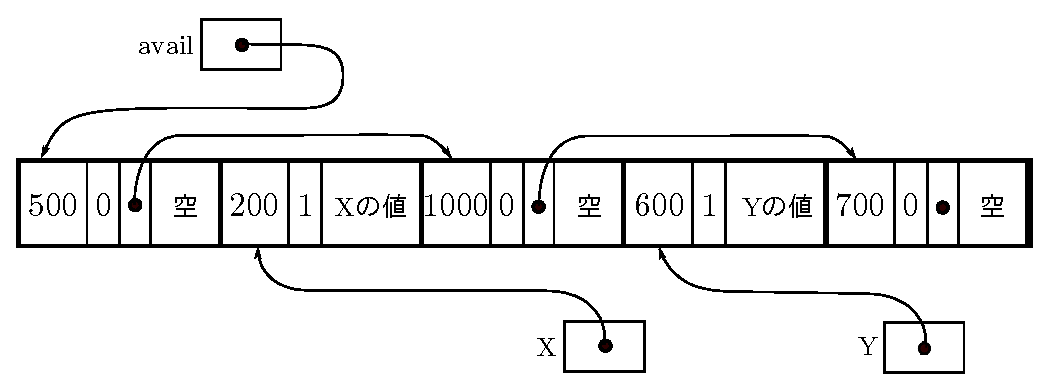
\includegraphics[scale=0.4]{../figures/eps/fig11.eps}
\caption{ヒープによる管理}
\label{fig11}
\end{figure}
%
新しいデータを入れるための空ブロックを探したり,不要になったデータが入っているブロックを再利用したりできるように本節ではブロックに関して次のように仮定する.
%
\begin{description}
  \item[(1)] 各ブロックは次のデータを格納するだけの大きさがあるものとする.
 \begin{description}
  \item[(a)] ブロックの大きさ
  \item[(b)] 使用可能なブロックをつなぐポインタ
  \item[(c)] ブロックが空かどうかを示すビット
 \end{description}
  \item[(2)] 空ブロックは左から,ブロックの長さ,0のFull/Empty ビット,次の使用可能ブロックへのポインタ,空領域という形をしている.
  \item[(3)] データを保有しているブロックは左から,長さ,1の Full/Empty ビット,データ自身という形をしている.
\end{description}
%
こうした仮定から,使用中はデータを入れることができ,使用してないときは同じ場所にポイントを入れる必要がある.
% このため,このようなブロックを扱うプログラムを書くには,Pascalなど強い型つけを行う言語は使えない,あるいは不便である.擬似的な Pascal のプログラムなら書けるが,本当の Pascal プログラムは書けない.ただし,アセンブリ言語や,C言語などのシステムプログラムなら問題ない.


\subsection{断片化と空ブロックの詰め直し}
%
ヒープ管理で生ずる特別な問題を調べるため,{\bf Fig.}{\ref{fig11}}で変数Yの値が変わり,それを表していたブロックを使用可能スペースにしたいときを考える.このブロックは,使用可能スペースリストの先頭に入れるのが最も楽である.

断片化とは,使用可能リスト上の大きな領域が小さなブロックの集まりになってしまう傾向をいう.こうして
空になったブロックを隣接する空ブロックとまとめることで断片化をおさえるには次の3つが挙げられる.
%
\begin{description}
  \item[(1)] ブロックが空くたびに隣接空領域をまとめる.
% 使用スペースリストをソートする.
% ブロックが空くたびに使用可能スペースの長さに比例した時間をかけ,隣接空領域をまとめる.
  \item[(2)] ブロックが空くたびに,双方向の使用可能スペースリストに登録する.
% その際,すべてのブロックに左隣へのポインタを持たせて隣接空領域を一定時間でまとめる.
  \item[(3)] 隣接空領域をまとめずにそのままにしておく.
\end{description}
%
%
\subsection{使用可能ブロックの選択}
%
新しいデータを格納するには,新たにブロックを提供する必要がある.そのためには,使用可能なブロックから1つを選び,その一部,または全部に新しいデータを入れる必要がある.
これらの選択に際して,
データを入れるブロックをなるべく早く,かつ断片化が進まないようにしたい.そのために以下の2つの方法がある.
%
\begin{description}
  \item[(1)] 初適合法:最初に見つけたブロックを選択する.
  \item[(2)] 最良適合法:ブロックの中で最小のブロックを\\~~~~~~~~~~~~~~~~~選択する.
\end{description}
%
% (1)の方法:
%  ・ブロックを素早く決められる.
%  ・
% (2)の方法:
%  ・使用可能スペースをすべて調べるため時間がかかる.→ ブロックの大きさごとに区別しておけば速くすることは可能.
%  ・(1)に比べ断片化を抑えられる.
%  ・半端になった非常に小さい断片を残す傾向がある.断片の数は(1)と変わらないが,占める領域は小さい.
%

(1)の方法は(2)の方法に比べ素早く決められる.(2)の方法は処理時間が圧倒的に遅いが,断片化を抑えられる.断片の数はあまり変わらないが,占める領域は小さい.ただし,これらの方法は中程度の大きさの断片をあまり作らないため,(1)なら応じられるものでも(2)では応じられないという傾向がある.その逆もしかりである.

\section{バディシステム}
%
断片化を防ぎながら,空ブロックの大きさの分布がひどくならないようにするデータを配置する方法であり,
隣接する空ブロックを短時間でまとめられる.一方で,ブロックの大きさが限られるため,必要以上の大きさのブロックを必要としてしまうことからスペースの無駄遣いが生じる.

バディシステムの考え方は,ブロックの大きさをいくつかの種類に制限することである.

$ s_1 ~<~ s_2 ~<~ s_3 ~<~ \cdots ~<~ s_k $という$ k $通りの大きさのブロックだけを使うものとする.
% これらに使われるのは 指数型バディシステム や フィボナッチ型 $ s_{i+1} = s_i + s_{i-1} $
この中から新しいデータが入る最小のブロックを使う.このときの大きさを$ s_i $とすると,この大きさの空ブロックがない場合は大きさ$ s_{i+1} $のブロックを探し,これを$ s_i $と$ s_{i+1} - s_i $の2つのブロックに分割する.
% バディ法では,$ s_{i+1} - s_i $がある$ j <= i $に対する$ s_j $と一致するようにしてある.このことから,sをどのように選んだかが分かる.
ある$ k \ge 0 $に対して$ j = i - k $であるとすると,$ s_{i+1} - s_i = s_{i-1} $より
%
\begin{equation*}
 s_{i+1} = s_i + s_{i-k}
\end{equation*}
%
が得られる.これを$ k $次のバディシステムという.特に,$ k = 0 $のときを指数型バディシステム,$ k = 1 $のときをフィボナッチバディシステムと呼ぶ.

\subsection{ブロックの分布}
%
$ k $次のバディシステムでは,大きさ$ s_{i+1} $のブロックは,$ s_i $と$ s_{i-k} $の2つのブロックからできていると考えられる.ここで,大きさ$ s_i $のブロックが左にあり,大きさ$ s_{i-k} $が右側にあるとすると,ヒープ全体がある大きな$ n $に対する1つのブロック$ s_n $であると考えられ,大きさ$ s_i $のブロックが始まる位置が決定される.
% 例を示す on slide


\subsection{ブロックの割り当て}
%
大きさ$ n $のブロックが必要になった場合,使用可能スペースリストから,$ n \le s_i $かつ$ i = 1 $または$ s_{i-1} < n $を満たす満たす大きさ$ s_i $のブロックをどれか1つ選び使用する.このような大きさのブロックがなければ,大きさ$ s_{i+1} $か$ s_{i+k+1} $のブロックを選んで分割すると,大きさ$ s_i $のブロックができる.そのようなブロックもなければ,$ s = {i+1} $の大きさについてこの分割法を再帰的に適用すればよい.

\subsection{ブロックの再利用}
%
ブロックが再度使用できるようになったとき,
%バディシステムの長所が発揮される.
新たに利用できるようになったブロックのバディも使用可能ならば,この2つをまとめることにより断片化を防ぐことができる.こうしてできたブロックがまた使用可能ならば,この2つもさらにまとめられ,この手順を繰り返すことができる.

指数型のバディシステムでは,バディの位置が簡単に分かるが,$ k \ge 1 $の場合は容易ではない.そのため,各ブロックに以下の情報を格納しておく.
%

\begin{description}
 \item[(1)] Full/Empty ビット
 \item[(2)] サイズインデックス:ブロックの大きさが$ s_i $で\\ ~~~~~~~~~~~~~~~~~~~~~~~~~~~~~あることを示す.
 \item[(3)] 左のバディカウント:そのブロックが何回連続で\\ ~~~~~~~~~~~~~~~~~~~~~~~~~~~~~~左側バディになるかを示す.
\end{description}
%
%詳細な説明(左バディカウントについて)が必要
%要推敲


\section{記憶の詰め直し}
%
空ブロックをまとめたとしても,新たな要求に応じられない場合がある.この問題の解決策として次の2つが挙げられる.
%
\begin{description}
 \item[(1)] いくつかの空ブロックをポインタでつないで使用する.
 \item[(2)] ヒープ内でデータを移動して使用中のブロックを左側に集め,右側に使用可能ブロックを1つにする.
\end{description}
%

(1)の方法はブロックをつなぐポインタ分にスペースを取られてしまうため,スペースの無駄遣いが起こりやすい.
一方で,比較的簡単に実現できるため,ほとんどのファイルシステムはこの方法を採用している.
(2)の方法は,効果は高いが,使用可能スペースをまとめるためにポインタの更新が必要であり多くの処理時間がかかる.
また,使用中のブロックの移動にはそのヒープの大きさに比例した時間がかかり,詰め直しのコストの中で最も大きな部分を占める.


\subsection{モリスのアルゴリズム}
%
ブロック内に移動先用のスペースを取らずにヒープを詰め直す方法である.使用中の各ブロック内の一定位置から始まるポインタの連鎖を作り,そのブロックを指しているポインタをすべてその連鎖につなげる.




% % 以下アクティビティ参考
% %-------------------------------
% \begin{equation}
% \mbox{\boldmath{$z$}} = f(x)\mbox{\boldmath{$a$}}
% %ベクトルaは\mbox{\boldmath{$a$} と書く.
% \label{eq:simple_z}
% \end{equation}
% %-------------------------------
% %-------------------------------
% \vspace{10mm}
% \begin{figure}[H]
% \centering
%   \includegraphics[scale=0.08]{../figures/evaluator.png}
% \caption{Grasp evaluator.}
% \label{fig:grasp_evaluator}
% \end{figure}
% %-------------------------------
% %-------------------------------
% \begin{spacing}{0.99}
% \begin{algorithm}[htbp]
% \caption{Random Grasp Planning}
% \label{alg:grasp}
% \nl Load learned CNN model : ${\rm CNN}(\mbox{\boldmath{$Image$}},\mbox{\boldmath{$Rectangle$}})$\\
% \nl Take an RGB color picture of the object : $\mbox{\boldmath{$I$}}_{\rm m}$\\
% \nl\While{${\rm true}$}{
% \nl Generate grasp rectangle randomly : $\mbox{\boldmath{$R$}}_{\rm rand}$\\
% \nl $N_{\rm out} \longleftarrow {\rm CNN}(\mbox{\boldmath{$I$}}_{\rm m},\mbox{\boldmath{$R$}}_{\rm rand})$\\
% \nl\If{$N_{\rm out} = {\rm true}$}{
% \nl ${\rm {\bf break}}$\\}}
% \nl $\mbox{\boldmath{$R$}}_{\rm out} \longleftarrow \mbox{\boldmath{$R$}}_{\rm rand}$\\
% \end{algorithm}
% \end{spacing}
% \vspace{-10mm}
% %-------------------------------
% %-------------------------------
% \begin{table}[H]
% \caption{Results of grasp planning.}
% \centering
% \vspace{4mm}
%   \begin{tabular}{|l|c|r||r|} \hline
%     メニュー & サイズ & 値段 & カロリー \\ \hline \hline
%     牛丼 & 並盛 & 500円 & 600 kcal \\
%     牛丼 & 大盛 & 1,000円 & 800 kcal \\
%     牛丼 & 特盛 & 1,500円 & 1,000 kcal \\ \hline
%     牛皿 & 並盛 & 300円 & 250 kcal \\
%     牛皿 & 大盛 & 700円 & 300 kcal \\
%     牛皿 & 特盛 & 1,000円 & 350 kcal \\ \hline
%   \end{tabular}
% \label{tb:gyudon}
% \end{table}
% %--------------------------------------------------------
% %-------------------------------
% \begin{thebibliography}{99}
% \addcontentsline{toc}{section}{参考文献}
% %-------------------------------
% \bibitem{text_nn} 岡谷貴之,『深層学習』(機械学習プロフェッショナルシリーズ),講談社, pp.7-33, pp.41-54, pp79-97, 2015.
% %-------------------------------
% \bibitem{IanLenz} Ian Lenz, Honglak Lee,
%  and Ashutosh Saxena.
%  ``Deep Learning for Detecting Robotic Grasps'',
%  The International Journal of Robotics Research,
%  34(4-5),pp.705-724, 2015.
% %-------------------------------
% \bibitem{PCL} PCL - Pint Cloud Library, accessed
%  10 February 2017, $<$\url{http://www.pointclouds.org/}$>$
% %-------------------------------
% \end{thebibliography}
\end{document}
